\chapter{Las reacciones químicas: reactivos y productos}\label{ch:g7:chemical-reactions}

El carbón vegetal brilla en una barbacoa. Una hora después, casi no
queda nada de los trozos negros: un poco de ceniza gris, y el calor que
ha cocinado la comida. ¿Adónde ha ido el carbono negro? No se ha
esfumado: se ha encontrado con el oxígeno del \omterm{def:g4:air-a-mixture-of-gases:air}{aire} y se ha convertido en
un gas nuevo e invisible. Ahora que conocemos los \omterm{def:g7:atoms-and-molecules:atom}{átomos} y las
\omterm{def:g7:atoms-and-molecules:molecule}{moléculas}, podemos decir con exactitud qué ocurre en un cambio así.

\begin{recall}
En un \omterm{def:g5:irreversible-changes:chemical-change}{cambio químico} aparecen sustancias nuevas y no hay un camino de
vuelta sencillo (\cref{ch:g5:irreversible-changes}). El agua de cal se
enturbia con el dióxido de carbono, y el sulfato de cobre anhidro se
vuelve azul con el agua (\cref{ch:g7:identifying-substances}). Toda la
materia está hecha de \omterm{def:g7:atoms-and-molecules:atom}{átomos}, que se agrupan en \omterm{def:g7:atoms-and-molecules:molecule}{moléculas}; una fórmula
como \ce{CO2} enumera los \omterm{def:g7:atoms-and-molecules:atom}{átomos} de una \omterm{def:g7:atoms-and-molecules:molecule}{molécula} (\cref{ch:g7:atoms-and-molecules}).
\end{recall}

\begin{omfigure}
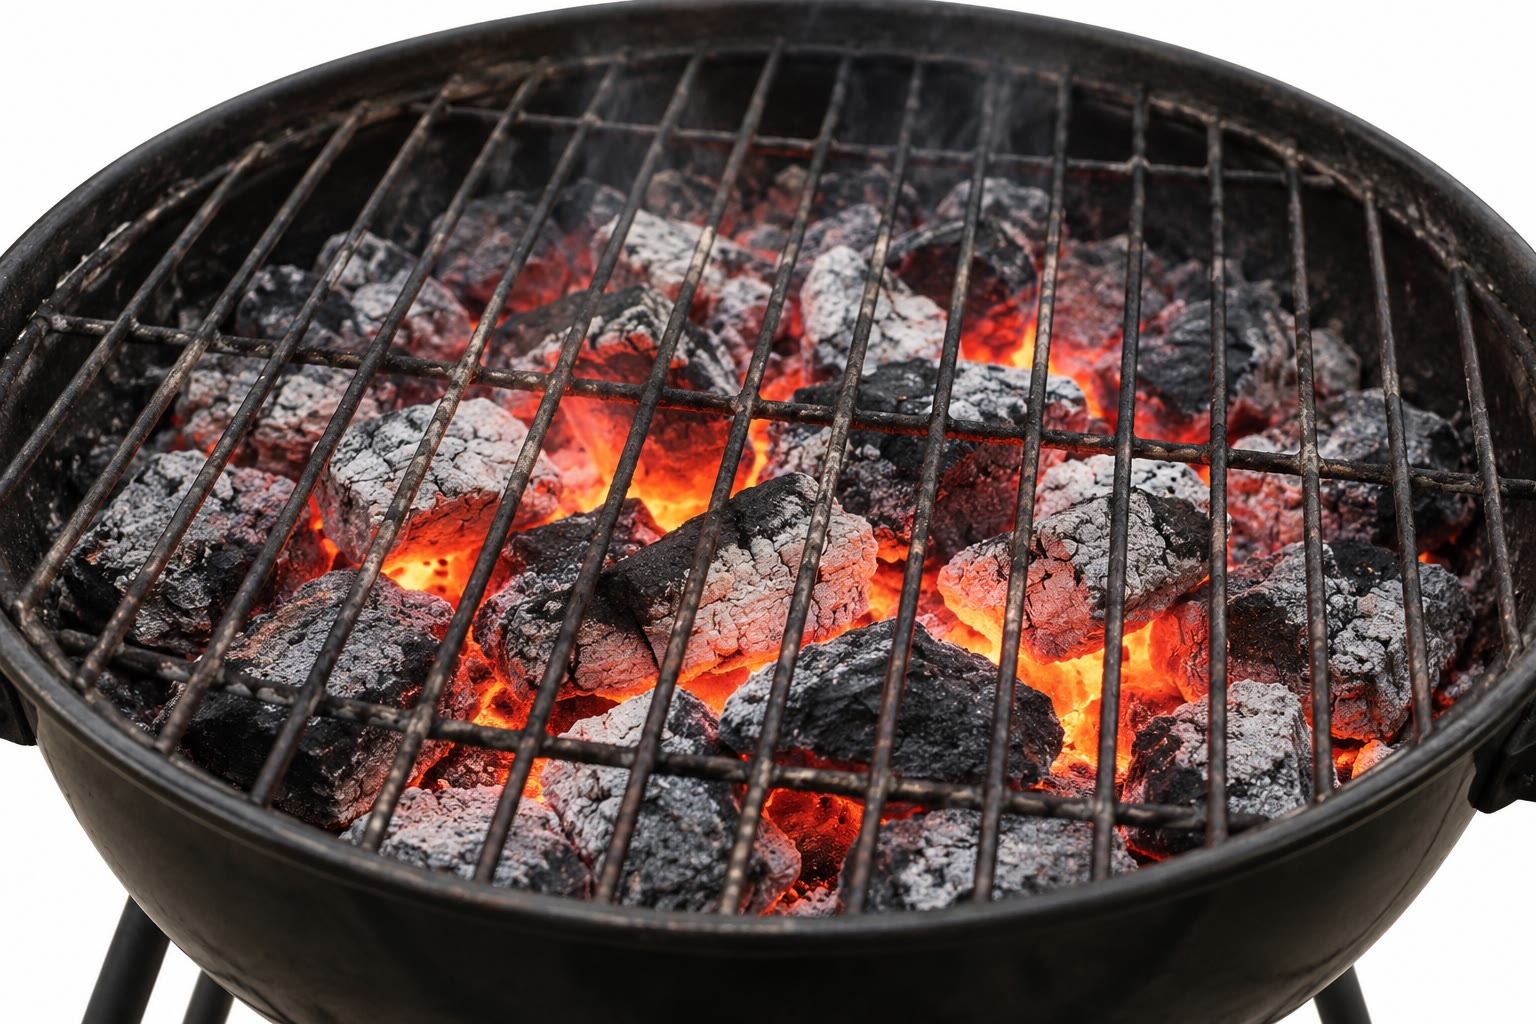
\includegraphics[width=0.55\linewidth]{images/book1/ai/g7-charcoal-bbq.jpg}

{\small Carbón incandescente: el carbono reacciona con el oxígeno del
\omterm{def:g4:air-a-mixture-of-gases:air}{aire}.}
\end{omfigure}

\section{Transformaciones físicas y químicas}

\begin{definition}[Transformación física]\label{def:g7:chemical-reactions:physical-transformation}
Una \emph{transformación física}\index{transformacion fisica@transformación física} cambia el
estado o la disposición de la materia sin cambiar las \omterm{def:g6:pure-substances-and-mixtures:species}{especies
químicas}: la fusión, la solidificación, la ebullición, la disolución, la
\omterm{def:g6:pure-substances-and-mixtures:mixture}{mezcla}. Antes y después están presentes las mismas especies; solo ha
cambiado su forma o su disposición.
\end{definition}

\begin{example}[El agua, de tres maneras]\label{ex:g7:chemical-reactions:water}
El hielo que se funde y se convierte en agua, el agua que hierve y se
convierte en vapor de agua y la sal que se \omterm{def:g2:mixing-and-dissolving:dissolve}{disuelve} en agua son
\omterm{def:g7:chemical-reactions:physical-transformation}{transformaciones físicas}: antes y después hay \omterm{def:g7:atoms-and-molecules:molecule}{moléculas} de agua (y
sal). Si hacemos zoom, las \omterm{def:g7:atoms-and-molecules:molecule}{moléculas} son las mismas; solo ha cambiado
cómo están dispuestas y cómo se mueven.
\end{example}

\begin{proposition}[Transformación química]\label{prop:g7:chemical-reactions:chemical}
En un \omterm{def:g5:irreversible-changes:chemical-change}{cambio químico}, llamado también transformación química,
desaparecen algunas \omterm{def:g6:pure-substances-and-mixtures:species}{especies químicas} y aparecen otras nuevas. Se
distingue de una \omterm{def:g7:chemical-reactions:physical-transformation}{transformación física} por sus \omterm{def:g7:chemical-reactions:reactant}{productos}: especies
nuevas, que se pueden detectar con \omterm{def:g7:identifying-substances:characteristic-test}{ensayos característicos}.
\end{proposition}

\begin{omfigure}
\begin{tikzpicture}[font=\small, level distance=1.5cm,
    box/.style={draw=omDef, fill=omDef!6, rounded corners=2pt, align=center,
      inner sep=4pt},
    level 1/.style={sibling distance=6.6cm},
    edge from parent/.style={draw, thick, omDef, ->}]
  \node[box] {una transformación de la materia}
    child {node[box, text width=5.2cm] {\textbf{física}: las mismas especies\\
      antes y después\\ \footnotesize fusión, ebullición, disolución, mezcla}}
    child {node[box, draw=omProp, fill=omProp!6, text width=5.2cm]
      {\textbf{química}: desaparecen especies,\\ aparecen especies nuevas\\
      \footnotesize combustión, oxidación, cocción}};
\end{tikzpicture}

{\small Dos clases de transformaciones.}
\end{omfigure}

\section{Reactivos y productos}

\begin{definition}[Reacción química]\label{def:g7:chemical-reactions:reaction}
Una \emph{reacción química}\index{reaccion quimica@reacción química} es el modelo que
usan los químicos para describir una transformación química: enumera
las especies que se consumen y las especies que se forman.
\end{definition}

\begin{definition}[Reactivos y productos]\label{def:g7:chemical-reactions:reactant}
Las especies que se consumen en una \omterm{def:g7:chemical-reactions:reaction}{reacción química} son los
\emph{reactivos}\index{reactivo}; las especies que se forman son los
\emph{productos}\index{producto}.
\end{definition}

\begin{example}[El carbono arde en oxígeno]\label{ex:g7:chemical-reactions:carbon}
Cuando \omterm{def:g4:what-a-fire-needs:burning}{arde} el carbón vegetal, los \omterm{def:g7:chemical-reactions:reactant}{reactivos} son el carbono (el carbón)
y el oxígeno (del \omterm{def:g4:air-a-mixture-of-gases:air}{aire}). El \omterm{def:g7:chemical-reactions:reactant}{producto} es el dióxido de carbono: agitado
con agua de cal, el gas que queda en el frasco la enturbia.
\end{example}

\begin{inthelab}[Carbón en un frasco de oxígeno]
El profesor calienta un trocito de carbón vegetal en una cucharilla de
\omterm{def:g4:what-a-fire-needs:burning}{combustión} hasta que se pone incandescente, y lo introduce en un frasco
de oxígeno. El carbón brilla mucho más que en el \omterm{def:g4:air-a-mixture-of-gases:air}{aire} y se va
reduciendo hasta desaparecer. Se tapa el frasco, se vierte un poco de
agua de cal y se agita: se enturbia. Se han consumido carbono y oxígeno;
se ha formado dióxido de carbono.
\end{inthelab}

\begin{omfigure}
\begin{tikzpicture}[font=\small, scale=1.3]
  \pic[transform shape] at (0,0) {gasjaropen={0}{white}};
  \fill[omWater!60] (-0.68,2.62) rectangle (0.68,2.7);
  \draw[omGlass, line width=0.4pt] (-0.68,2.62) rectangle (0.68,2.7);
  \draw[black!60, line width=1.2pt] (0.15,2.7) -- (0.15,3.6) -- (1.2,3.6);
  \draw[black!60, line width=1.2pt] (0.15,2.7) -- (0.15,1.2);
  \fill[black!60] (-0.12,1.12) rectangle (0.32,1.2);
  \fill[red!70!black] (0.0,1.32) circle (0.13);
  \fill[orange!90!yellow] (0.0,1.32) circle (0.08);
  \draw[<-, omProp, thick] (0.15,1.35) -- (1.5,1.6) node[right, text=black]
    {carbón incandescente (carbono)};
  \draw[<-, omProp, thick] (-0.35,2.1) -- (1.5,2.3) node[right, text=black]
    {oxígeno};
  \draw[<-, omProp, thick] (0.6,2.66) -- (1.5,2.95) node[right, text=black]
    {tapa};
  \draw[<-, omProp, thick] (0.15,3.1) -- (1.5,3.6) node[right, text=black]
    {cucharilla de combustión};
\end{tikzpicture}

{\small Un trozo de carbón incandescente introducido con una cucharilla
en un frasco de oxígeno \omterm{def:g4:what-a-fire-needs:burning}{arde} con viveza: el carbono y el oxígeno
reaccionan y forman dióxido de carbono.}
\end{omfigure}

\begin{example}[La lana de acero]\label{ex:g7:chemical-reactions:steel-wool}
Un estropajo de lana de acero fina, que es sobre todo hierro, puede
\omterm{def:g4:what-a-fire-needs:burning}{arder} en el \omterm{def:g4:air-a-mixture-of-gases:air}{aire} lanzando lluvias de chispas. Los \omterm{def:g7:chemical-reactions:reactant}{reactivos} son el
hierro y el oxígeno; el \omterm{def:g7:chemical-reactions:reactant}{producto} es un sólido oscuro y quebradizo, un
óxido de hierro.
\end{example}

\begin{omfigure}
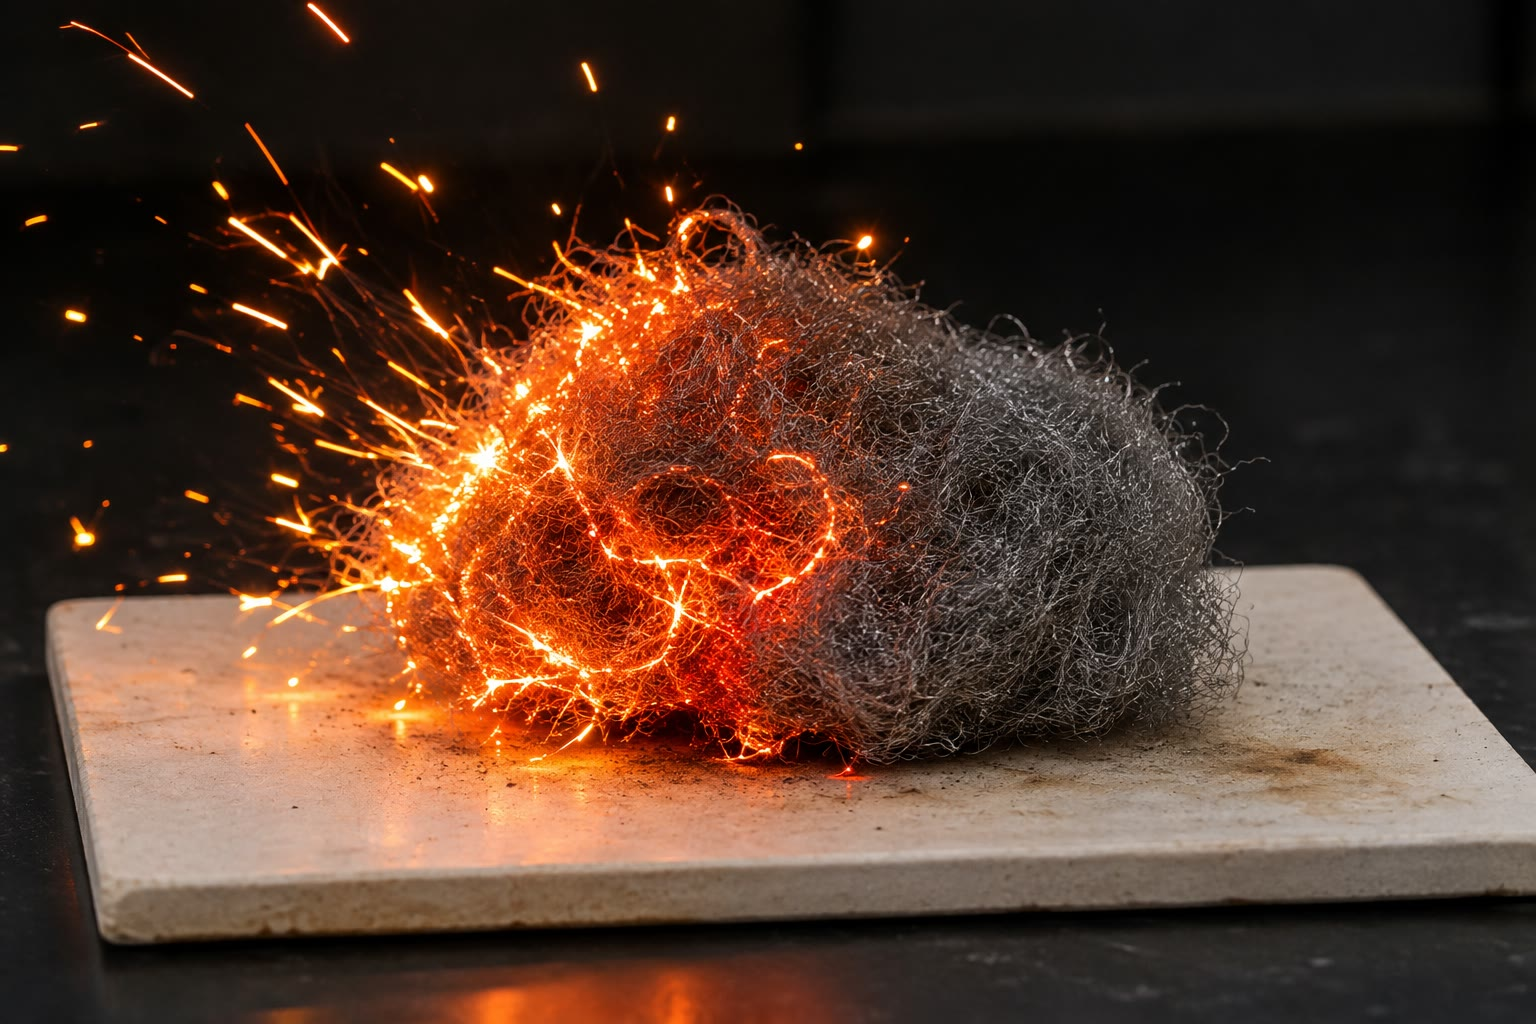
\includegraphics[width=0.5\linewidth]{images/book1/ai/g7-steel-wool-burning.jpg}

{\small Lana de acero \omterm{def:g4:what-a-fire-needs:burning}{ardiendo} en el laboratorio: el hierro y el oxígeno
reaccionan.}
\end{omfigure}

\section{La ecuación con palabras}

\begin{definition}[Ecuación con palabras]\label{def:g7:chemical-reactions:word-equation}
Una \emph{ecuación con palabras}\index{ecuacion con palabras@ecuación con palabras} escribe
una \omterm{def:g7:chemical-reactions:reaction}{reacción química} con palabras: los nombres de los \omterm{def:g7:chemical-reactions:reactant}{reactivos} a la
izquierda, unidos por $+$, una flecha, y los nombres de los \omterm{def:g7:chemical-reactions:reactant}{productos} a
la derecha. La flecha se lee ``reaccionan y dan''.
\end{definition}

\begin{example}[Tres ecuaciones con palabras]\label{ex:g7:chemical-reactions:three}
\begin{center}
\begin{tabular}{l}
carbono $+$ oxígeno $\longrightarrow$ dióxido de carbono\\[2pt]
metano $+$ oxígeno $\longrightarrow$ dióxido de carbono $+$ agua\\[2pt]
hierro $+$ oxígeno $\longrightarrow$ óxido de hierro
\end{tabular}
\end{center}
\end{example}

\begin{method}[Escribir una ecuación con palabras]\label{met:g7:chemical-reactions:write}
\begin{enumerate}
  \item Buscar los \omterm{def:g7:chemical-reactions:reactant}{reactivos}: las especies que desaparecen.
  \item Buscar los \omterm{def:g7:chemical-reactions:reactant}{productos}: las especies nuevas, identificadas
        mediante ensayos.
  \item Escribir los \omterm{def:g7:chemical-reactions:reactant}{reactivos} a la izquierda y los \omterm{def:g7:chemical-reactions:reactant}{productos} a la
        derecha, con una flecha entre ellos; nunca un signo igual.
\end{enumerate}
Una especie que está presente pero no participa (el nitrógeno del \omterm{def:g4:air-a-mixture-of-gases:air}{aire}
que rodea una llama) no se escribe.
\end{method}

\section{Una reacción es una reorganización de átomos}

\begin{proposition}[Los átomos se reorganizan]\label{prop:g7:chemical-reactions:rearranged}
En una \omterm{def:g7:chemical-reactions:reaction}{reacción química}, las \omterm{def:g7:atoms-and-molecules:molecule}{moléculas} de los \omterm{def:g7:chemical-reactions:reactant}{reactivos} se rompen y sus
\omterm{def:g7:atoms-and-molecules:atom}{átomos} se unen de otra manera para construir las \omterm{def:g7:atoms-and-molecules:molecule}{moléculas} de los
\omterm{def:g7:chemical-reactions:reactant}{productos}. Los \omterm{def:g7:atoms-and-molecules:atom}{átomos} mismos ni se crean ni se destruyen: antes y
después están los mismos \omterm{def:g7:atoms-and-molecules:atom}{átomos}, en el mismo número.
\end{proposition}

\begin{example}[El metano arde, molécula a molécula]\label{ex:g7:chemical-reactions:methane}
Cuando \omterm{def:g4:what-a-fire-needs:burning}{arde} el metano de una cocina de gas, una \omterm{def:g7:atoms-and-molecules:molecule}{molécula} de metano
\ce{CH4} se encuentra con dos \omterm{def:g7:atoms-and-molecules:molecule}{moléculas} de oxígeno \ce{O2}. Sus \omterm{def:g7:atoms-and-molecules:atom}{átomos}
se reorganizan en una \omterm{def:g7:atoms-and-molecules:molecule}{molécula} de dióxido de carbono \ce{CO2} y dos
\omterm{def:g7:atoms-and-molecules:molecule}{moléculas} de agua \ce{H2O}. Antes: 1 \omterm{def:g7:atoms-and-molecules:atom}{átomo} de carbono, 4 de hidrógeno y
4 de oxígeno. Después: 1 de carbono, 4 de hidrógeno y $2 + 2 = 4$ de
oxígeno. No se pierde nada, y nada aparece de la nada.
\end{example}

\begin{omfigure}
\begin{tikzpicture}[font=\small]
  % methane
  \begin{scope}[xshift=0cm]
    \node[aC] (c) at (0,0) {};
    \node[aH] (h1) at (0,0.78) {}; \node[aH] (h2) at (-0.74,-0.3) {};
    \node[aH] (h3) at (0.74,-0.3) {}; \node[aH] (h4) at (0.2,-0.68) {};
    \begin{scope}[on background layer]
      \foreach \h in {h1,h2,h3,h4} \draw[bond] (c.center) -- (\h.center);
    \end{scope}
    \node at (0,-1.2) {1 metano};
  \end{scope}
  \node at (1.45,0) {$+$};
  % two oxygen molecules
  \foreach \y in {0.45,-0.45} {
    \node[aO] (a) at (2.4,\y) {}; \node[aO] (b) at (3.05,\y) {};
    \begin{scope}[on background layer]
      \draw[bond, line width=1.1pt] ([yshift=1.6pt]a.center) -- ([yshift=1.6pt]b.center);
      \draw[bond, line width=1.1pt] ([yshift=-1.6pt]a.center) -- ([yshift=-1.6pt]b.center);
    \end{scope}
  }
  \node at (2.72,-1.2) {2 oxígeno};
  \draw[->, thick, omProp] (3.8,0) -- (5.0,0);
  % carbon dioxide
  \begin{scope}[xshift=6.3cm]
    \node[aO] (a) at (-0.8,0) {}; \node[aC] (c) at (0,0) {}; \node[aO] (b) at (0.8,0) {};
    \begin{scope}[on background layer]
      \foreach \d in {-1.6,1.6} {
        \draw[bond, line width=1.1pt] ([yshift=\d pt]a.center) -- ([yshift=\d pt]c.center);
        \draw[bond, line width=1.1pt] ([yshift=\d pt]c.center) -- ([yshift=\d pt]b.center);}
    \end{scope}
    \node at (0,-1.2) {1 dióxido de carbono};
  \end{scope}
  \node at (7.8,0) {$+$};
  % two water molecules
  \foreach \x in {8.9,10.6} {
    \node[aO] (o) at (\x,0.2) {};
    \node[aH] (p) at (\x-0.58,-0.25) {}; \node[aH] (q) at (\x+0.58,-0.25) {};
    \begin{scope}[on background layer]
      \draw[bond] (o.center) -- (p.center); \draw[bond] (o.center) -- (q.center);
    \end{scope}
  }
  \node at (9.75,-1.2) {2 agua};
  % atom counts
  \node[align=center, font=\footnotesize] at (1.5,-2.0) {antes: 1 C, 4 H, 4 O};
  \node[align=center, font=\footnotesize] at (8.5,-2.0) {después: 1 C, 4 H, 4 O};
\end{tikzpicture}

{\small La \omterm{def:g4:what-a-fire-needs:burning}{combustión} del metano, dibujada con modelos moleculares: los
\omterm{def:g7:atoms-and-molecules:atom}{átomos} de los \omterm{def:g7:chemical-reactions:reactant}{reactivos} se reorganizan en los \omterm{def:g7:chemical-reactions:reactant}{productos}. Antes y después
se cuentan los mismos \omterm{def:g7:atoms-and-molecules:atom}{átomos}.}
\end{omfigure}

\begin{remark}[Contar las moléculas]\label{rem:g7:chemical-reactions:counting}
La \omterm{def:g7:chemical-reactions:word-equation}{ecuación con palabras} no dice cuántas \omterm{def:g7:atoms-and-molecules:molecule}{moléculas} reaccionan: para eso
se escribe la ecuación con fórmulas y con números delante de ellas.
Escribir esas ecuaciones, y encontrar los números correctos, es el tema
de un capítulo posterior.
\end{remark}

\section{Ejercicios}

\begin{exercise}[$\star$]\label{exo:g7:chemical-reactions:1}
¿\omterm{def:g7:chemical-reactions:physical-transformation}{Transformación física} o química? El hielo que se funde, una cerilla que
\omterm{def:g4:what-a-fire-needs:burning}{arde}, el azúcar que se \omterm{def:g2:mixing-and-dissolving:dissolve}{disuelve}, el pan que se tuesta, un clavo que se
oxida.
\end{exercise}

\begin{exercise}[$\star$]\label{exo:g7:chemical-reactions:2}
¿Qué son los \omterm{def:g7:chemical-reactions:reactant}{reactivos} y los \omterm{def:g7:chemical-reactions:reactant}{productos} de una \omterm{def:g7:chemical-reactions:reaction}{reacción química}?
\end{exercise}

\begin{exercise}[$\star$]\label{exo:g7:chemical-reactions:3}
Escribe la \omterm{def:g7:chemical-reactions:word-equation}{ecuación con palabras} de la \omterm{def:g4:what-a-fire-needs:burning}{combustión} del carbono en
oxígeno.
\end{exercise}

\begin{exercise}[$\star$]\label{exo:g7:chemical-reactions:4}
En la \omterm{def:g7:chemical-reactions:word-equation}{ecuación con palabras} ``hierro $+$ oxígeno $\longrightarrow$
óxido de hierro'', nombra los \omterm{def:g7:chemical-reactions:reactant}{reactivos} y el \omterm{def:g7:chemical-reactions:reactant}{producto}.
\end{exercise}

\begin{exercise}[$\star\star$]\label{exo:g7:chemical-reactions:5}
Cuando \omterm{def:g4:what-a-fire-needs:burning}{arde} el metano, un vaso frío sostenido encima de la llama se
empaña, y el gas recogido enturbia el agua de cal. ¿Qué \omterm{def:g7:chemical-reactions:reactant}{productos}
muestran estos dos ensayos?
\end{exercise}

\begin{exercise}[$\star\star$]\label{exo:g7:chemical-reactions:6}
El cinc reacciona con el ácido clorhídrico: el cinc desaparece, se
desprenden burbujas de hidrógeno y el cloruro de cinc queda en la
disolución. Escribe la \omterm{def:g7:chemical-reactions:word-equation}{ecuación con palabras}.
\end{exercise}

\begin{exercise}[$\star\star$]\label{exo:g7:chemical-reactions:7}
Mira la figura de los modelos de la \omterm{def:g4:what-a-fire-needs:burning}{combustión} del metano. Cuenta los
\omterm{def:g7:atoms-and-molecules:atom}{átomos} de hidrógeno antes y después de la reacción.
\end{exercise}

\begin{exercise}[$\star\star$]\label{exo:g7:chemical-reactions:8}
¿Por qué \omterm{def:g2:mixing-and-dissolving:dissolve}{disolver} sal en agua no es una \omterm{def:g7:chemical-reactions:reaction}{reacción química}, aunque la sal
desaparezca de la vista?
\end{exercise}

\begin{exercise}[$\star\star$]\label{exo:g7:chemical-reactions:9}
Un tronco de madera \omterm{def:g4:what-a-fire-needs:burning}{arde} hasta quedar reducido a un montoncito de
ceniza. Explica, usando la palabra ``\omterm{def:g7:chemical-reactions:reactant}{productos}'', por qué la ceniza es
mucho más ligera que el tronco.
\end{exercise}

\begin{exercise}[$\star\star$]\label{exo:g7:chemical-reactions:10}
El hidrógeno \omterm{def:g4:what-a-fire-needs:burning}{arde} en oxígeno y solo da agua. Escribe la \omterm{def:g7:chemical-reactions:word-equation}{ecuación con
palabras} y di qué ensayo identificaría el \omterm{def:g7:chemical-reactions:reactant}{producto}.
\end{exercise}

\begin{exercise}[$\star\star\star$]\label{exo:g7:chemical-reactions:11}
Dos \omterm{def:g7:atoms-and-molecules:molecule}{moléculas} de hidrógeno \ce{H2} reaccionan con una \omterm{def:g7:atoms-and-molecules:molecule}{molécula} de
oxígeno \ce{O2} y dan dos \omterm{def:g7:atoms-and-molecules:molecule}{moléculas} de agua \ce{H2O}. Cuenta los \omterm{def:g7:atoms-and-molecules:atom}{átomos}
de cada clase antes y después, y muestra que no se ha creado ni
destruido ninguno.
\end{exercise}

\begin{exercise}[$\star\star\star$]\label{exo:g7:chemical-reactions:12}
Un alumno dibuja la \omterm{def:g4:what-a-fire-needs:burning}{combustión} del carbono así: un \omterm{def:g7:atoms-and-molecules:atom}{átomo} de carbono $+$
una \omterm{def:g7:atoms-and-molecules:molecule}{molécula} de oxígeno $\longrightarrow$ una \omterm{def:g7:atoms-and-molecules:molecule}{molécula} de dióxido de
carbono y un \omterm{def:g7:atoms-and-molecules:atom}{átomo} de oxígeno que sobra. ¿Qué está mal en este dibujo?
Describe con palabras el dibujo correcto.
\end{exercise}

\section{Problema: Dentro de la llama de una cocina de gas}

\begin{problem}[{Problema de fin de semana --- qué arde en la llama de
una cocina de gas, qué produce y cuántas moléculas intervienen}]
\label{pb:g7:chemical-reactions:1}
El gas de una cocina es sobre todo metano, \ce{CH4}. En su llama azul,
el metano reacciona con el oxígeno del \omterm{def:g4:air-a-mixture-of-gases:air}{aire}. En un laboratorio, el
profesor sostiene durante unos segundos un vaso de precipitados frío y
seco, boca abajo, encima de una llama así; luego le da la vuelta, vierte
un poco de agua de cal y lo agita.

\medskip
\noindent\textbf{Parte I --- \omterm{def:g7:chemical-reactions:reactant}{Reactivos} y \omterm{def:g7:chemical-reactions:reactant}{productos}.}
\begin{enumerate}
  \item Nombra los dos \omterm{def:g7:chemical-reactions:reactant}{reactivos} de esta reacción.
  \item Dentro del vaso frío aparecen gotitas; una de ellas vuelve azul
        el sulfato de cobre anhidro. ¿Qué \omterm{def:g7:chemical-reactions:reactant}{producto} muestra esto?
  \item El agua de cal se enturbia. ¿Qué otro \omterm{def:g7:chemical-reactions:reactant}{producto} muestra esto?
  \item El \omterm{def:g4:air-a-mixture-of-gases:air}{aire} contiene también nitrógeno, que atraviesa la llama sin
        cambiar. ¿Es el nitrógeno un \omterm{def:g7:chemical-reactions:reactant}{reactivo}? ¿Debe aparecer en la
        \omterm{def:g7:chemical-reactions:word-equation}{ecuación con palabras}?
\end{enumerate}

\medskip
\noindent\textbf{Parte II --- La \omterm{def:g7:chemical-reactions:word-equation}{ecuación con palabras}.}
\begin{enumerate}[resume]
  \item Escribe la \omterm{def:g7:chemical-reactions:word-equation}{ecuación con palabras} de la reacción.
  \item ¿La \omterm{def:g4:what-a-fire-needs:burning}{combustión} del metano es una \omterm{def:g7:chemical-reactions:physical-transformation}{transformación física} o
        química? Da dos razones.
  \item Escribe las fórmulas de las cuatro especies de la reacción.
\end{enumerate}

\medskip
\noindent\textbf{Parte III --- Contar \omterm{def:g7:atoms-and-molecules:molecule}{moléculas}.}
Cada \omterm{def:g7:atoms-and-molecules:molecule}{molécula} de metano que \omterm{def:g4:what-a-fire-needs:burning}{arde} reacciona con dos \omterm{def:g7:atoms-and-molecules:molecule}{moléculas} de oxígeno
y da una \omterm{def:g7:atoms-and-molecules:molecule}{molécula} de dióxido de carbono y dos \omterm{def:g7:atoms-and-molecules:molecule}{moléculas} de agua.
\begin{enumerate}[resume]
  \item Cuenta los \omterm{def:g7:atoms-and-molecules:atom}{átomos} de carbono, de hidrógeno y de oxígeno que hay
        en una \omterm{def:g7:atoms-and-molecules:molecule}{molécula} de metano y dos \omterm{def:g7:atoms-and-molecules:molecule}{moléculas} de oxígeno, juntas.
  \item Cuéntalos en una \omterm{def:g7:atoms-and-molecules:molecule}{molécula} de dióxido de carbono y dos \omterm{def:g7:atoms-and-molecules:molecule}{moléculas}
        de agua, juntas. ¿Qué observas?
  \item La llama quema 10 \omterm{def:g7:atoms-and-molecules:molecule}{moléculas} de metano. ¿Cuántas \omterm{def:g7:atoms-and-molecules:molecule}{moléculas} de
        oxígeno consume?
  \item ¿Cuántas \omterm{def:g7:atoms-and-molecules:molecule}{moléculas} de dióxido de carbono produce?
  \item ¿Cuántas \omterm{def:g7:atoms-and-molecules:molecule}{moléculas} de agua produce?
\end{enumerate}
\end{problem}
